\subsection{Systemarchitektur}

\subsubsection{Contiki}
Contiki ist ein Open Source Echtzeitbetriebssystem, das bei uns in der PG auf den MICAz-Modulen eingesetzt wird.
Contiki bietet einen einfachen ereignisgesteuerten Betriebssystemkern mit sogenannten Protothreads, optionalem 
pr\"aemptiven Multiprogramming, Interprozesskommunikation via Messagepassing durch Events, eine dynamische Prozessstruktur
mit Unterst\"utzung f\"ur das Laden und Entladen von Programmen, nativen TCP/IP-Support über den uIP TCP/IP-Stack und eine 
grafische Benutzerschnittstelle, welche direkt auf einem Bildschirm oder als virtuelle Anzeige \"uber Telnet oder VNC genutzt werden kann \cite{Wikipedia:2013:Online}.
 
\paragraph{Systemarchitektur}
Ein laufendes Contiki System besteht aus dem Kernel, Bibliotheken, Prozessen und dem Programm-Lader, mit dem Anwendungen zur Laufzeit aus dem Speicher oder \"uber ein Funkmodul geladen werden k\"onnen.
Die unten stehende Abbildung zeigt die Aufteilung des Betriebssystems in zwei Teile. 
\begin{figure}[h!]
	\centering
		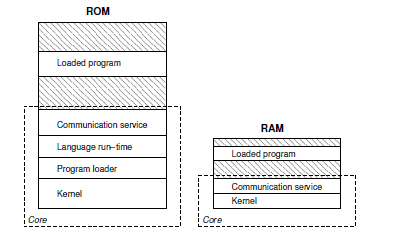
\includegraphics[width=0.9\textwidth]{Systemarchitektur_Contiki.png}
	\caption{Komponenten von Contiki \cite{Dunkels:Groenvall:Voigt:2014:Online}}
	\label{Systemarchitektur von Contiki}
\end{figure}
Der Core ist ein Basissystem und besteht aus dem Kernel, Bibliotheken, Ger\"{a}tetreibern und dem Programm-Lader. 
Im allgemeinen sind \"Anderungen am Core nicht vorgesehen und nur unter Verwendung eines speziellen Bootloaders m\"oglich. 
Die konkrete Aufteilung des Systems in Core und ladbare Programme wird beim Kompilieren des Systems entschieden und h\"angt 
von der Hardware-Plattform ab \cite[vgl.][S. 7]{Walter:2010}. Ger\"atetreiber werden als Bibliotheken implementiert. 

\paragraph{Events}
In Contiki kommunizieren Prozesse \"uber Events. Auch der Kernel versendet Events, um Prozesse \"uber ihren Status 
(Init, Continue, Exit) oder \"uber abgelaufene Timer zu Informieren. Zur Identifikation stehen dabei Event IDs zur 
Verf\"ugung. Die Event IDs 0-127 k\"onnen vom Benutzer frei vergeben werden, w\"ahrend die Prozess IDs ab 128 vom 
System genutzt werden. Grunds\"atzlich unterscheidet Contiki zwischen synchronen und asynchronen Events. 
\begin{itemize}
\item \textbf{Asynchrone Events} sind eine Form der Deferred Procedure Call: asynchrone Events werden vom Kernel in einer 
Warteschlange gespeichert. Die Scheduling-Funktion des Kernels l\"auft nach Systemstart in einer Endlosschleife. 
In jedem Durchlauf wird ein Event aus der Schlange entnommen und wird einige Zeit sp\"ater an den Zielprozess weitergeleitet.
\item \textbf{Synchrone Events} gleichen einem Funktionsaufruf.
Sie werden ohne Umweg \"uber die Warteschlange direkt an den Empf\"anger-Prozess
zugestellt \cite[vgl.][S. 7]{Walter:2010}.  Mit der Funktion process\_post\_synch(\&example\_process, EVENT\_ID, msg) wird gezielt ein 
Prozess aufgerufen (ein Broadcast ist nicht m\"oglich). W\"ahrend der aufgerufene Prozess aktiv ist, blockiert der Aufrufer und 
setzt seine Ausführung erst fort, wenn der aufgerufene Prozess die Kontrolle wieder abgibt.
\end{itemize}

\paragraph{Prozesse}
Prozesse in Contiki implementieren ein Konzept namens Protothreads. Dies erlaubt es Prozessen, ohne den Overhead und die langen 
Prozesswechselzeiten von normalen Threads auszukommen. Gleichzeitig k\"onnen trotzdem andere Prozesse ausgef\"uhrt werden, falls ein Prozess auf ein Event (Timer, Nachricht von anderem Prozess...) warten muss.
F\"ur die Entwicklung mit Prozessen ist wichtig, dass nicht-statische Variablen nicht zwischen zwei Aufrufen erhalten bleiben.
Der relevante Status eines Prozesses sollte daher mithilfe von statischen Variablen abgelegt werden (siehe Variable i im folgenden Beispiel)

\begin{figure}[h!]
	\centering
		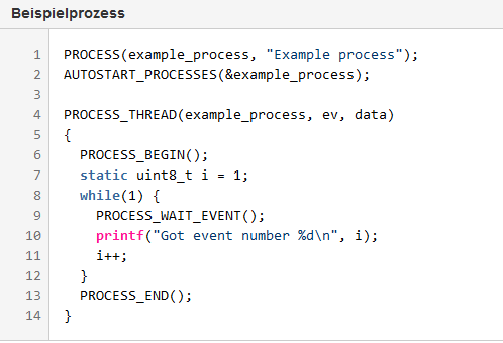
\includegraphics[width=0.9\textwidth]{Beispielprozess.png}
	\label{Beispielprozess}
\end{figure}
In Zeile 1 wird der Prozess initialisiert und in Zeile 2 automatisch beim Boot von Contiki gestartet. Zeile 4 beinhaltet die
Deklaration. So k\"onnen andere Prozesse diesem Prozess Events (mit oder ohne Daten) schicken, auf die unser Beispielprozess 
mit ev und data zugreifen kann. Zeile 6 kennzeichnet den Beginn der tats\"achlichen Ablauflogik. Code \"uber dieser Zeile wird 
bei jedem Prozessaufruf ausgef\"uhrt, dies wird jedoch in den meisten F\"allen nicht ben\"otigt. Zeile 13 schlie{\ss}lich beendet
den Prozess und entfernt ihn aus der Prozess-Liste des Kernels. In diesem Beispiel wird die Zeile jedoch nie erreicht, sodass der Prozess immer wieder aufgerufen wird, bis er von einem anderen Prozess beendet wird.
Wichtige Funktionen in Prozessen:
\begin{itemize}
\item PROCESS\_WAIT\_EVENT() - Wartet auf ein beliebiges Event, bevor die Ausf\"{u}hrung fortgesetzt wird.
\item PROCESS\_WAIT\_EVENT\_UNTIL(condition) - Wartet auf ein beliebiges Event, setzt die Ausf\"{u}hrung aber nur fort, wenn die Bedingung erf\"{u}llt ist.
\item PROCESS\_WAIT\_UNTIL() - Wartet, bis die Bedingung erf\"ullt ist. Muss den Prozess nicht zwangsl\"{a}ufig anhalten.
\end{itemize}
Prozesse k\"onnen \"uber Events (siehe Events) oder Polling-Anfragen kommunizieren.  Polls sind Events mit hoher Priorit\"at und 
k\"onnen genutzt werden, um den angerufenen Prozess so schnell wie m\"oglich auszuf\"uhren. Sie
sind besonders bei der Abarbeitung von Hardware-Interrupts wichtig, da Interrupts-Handler keine Events, sondern nur
Polling-Anfragen absetzten d\"urfen \cite[vgl.][S. 7]{Walter:2010}.

\subsubsection{Treiber, Services und Interfaces}
Auf dieser Ebene werden der Agenten RTE alle Funktionalitäten zur Verfügung gestellt. Das RTOS stellt Infrastruktur wie z.~B. Task Management, Timing, Events usw.
Die Driver Ebene kümmert sich um die Schnittstellen/Pins des Controllers wie z.~B. Protokolle angeschlossener
Devices\cite[S. 26]{Stasch:Hahn}. Die Aufgabe des Service ist es, Funktionen für spezielle Anwendungen zur Verfügung zu stellen.
Darüber kommen die Interfaces. Diese sind nötig, damit bestimmte Funktionen immer gleich der Agenten RTE zur Verfügung gestellt werden, auch wenn der Service anders ist oder wenn ein Service verschiedene Interfaces bedienen soll\cite[S. 26]{Stasch:Hahn}.

\subsubsection{Agenten RTE}

Zur Umsetzung der dezentralen Steuerung werden Softwareagenten eingesetzt. Bei Software-Agenten handelt es sich um Prozesse, die lose gekoppelt 
und leicht austauschbar sind \cite[vgl.][S. 31-37]{GH:2010}. Es existieren verschiedene Definitionen eines Agenten, von denen
sich keine als Standard etablieren konnte. Die hier verwendete Definition stammt von
Brenner, Zarnekow und Wittig. Sie definieren einen Agenten als „ ... ein Softwareprogramm,
das für einen Benutzer bestimmte Aufgaben erledigen kann und dabei einen Grad an
Intelligenz besitzt, der es befähigt, seine Aufgaben in Teilen autonom durchzuführen und mit
seiner Umwelt auf sinnvolle Art und Weise zu interagieren“\cite{BZW:1998}. Die Fähigkeit von Agenten, miteinander zu kommunizieren 
und zu interagieren, ermöglicht das Erstellen eines Multiagentensystems (MAS). Ein wesentlicher Vorteil von MAS 
bzw. von verteilten Steuerungssystemen ist die Fähigkeit, dynamisch auf Veränderungen zu reagieren. Ein Beispiel für eine solche Veränderung ist der
Ausfall einer Steuerungseinheit bzw. eines Agenten. Der Ausfall einer Einheit hat nicht unbedingt zur Folge, dass das gesamte System ausfällt. 
Die restlichen Einheiten können sich eigenständig auf eine solche Veränderung einstellen und diese beim weiteren Ablauf
berücksichtigen\cite[S. 13]{Roidl:2012}. Diese Eigenschaft bringt eine ganze Reihe von Vorteilen für ein dezentral
gesteuertes Materialflusssystem mit sich.\\
Die Modellierung von agentenbasierten Systemen für industrielle Bereiche wird durch die
Entwicklung von Standards festgelegt. Diese beschreiben Modelle für die Architektur
sowie die Kommunikation zwischen Agenten. Die FIPA (Foundation of Intelligent Physical Agents) ist das Standardisierungsorgan für Agentensysteme.
Seit der Gründung 1996 in der Schweiz wurden verschiedene Standardisierungen veröffentlicht, so zum Beispiel auch die Agentenkommunikation (Agent Communication), die als FIPA/ACL (Agent Communication Language, ACL) bekannt geworden ist. Jeder Agent ist mit einem eindeutigen
Identifikationsnamen (Agent Identifier oder AID) versehen und wird im Agent Management System verwaltet\cite[S. 24]{Roidl:2012}.
Ein Verzeichnisdienst kann optional vom Directory Facilitator gestellt
werden. Die Komponenten sind über das Message Transport System (MTS) verbunden,
sodass alle Komponenten untereinander kommunizieren können\cite[S. 24]{Roidl:2012}. \\
Als Referenzmodell zur Verwaltung von Softwareagenten wurde die Softwarearchitektur der Materialflussgruppe laut den FIPA Standards aufgebaut. 
Die nächste Abbildung zeigt den Aufbau der Softwarearchitektur und ist an die AUTOSAR Softwarearchitektur angelehnt:
\begin{figure}[h!]
	\centering
		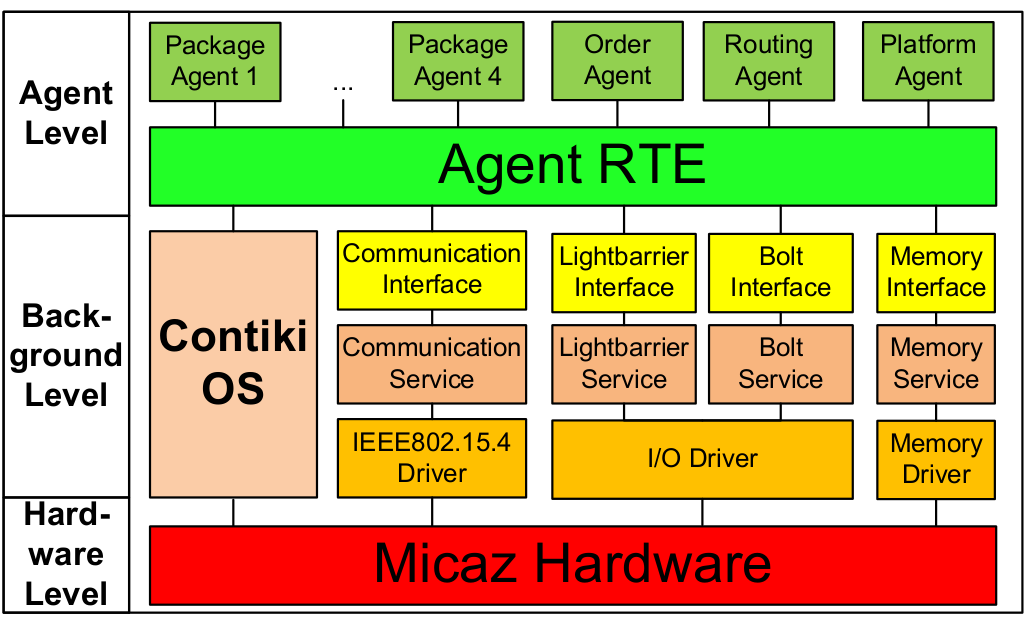
\includegraphics[width=0.9\textwidth]{ArchitekturMicazRampe.png}
	\caption{Architektur Micaz Rampe\cite{Stasch:Hahn}}
	\label{ArchitekturMicazRampe}
\end{figure}
\paragraph{Hardware Level}
Auf der Hardwareebene werden die Treiber für die Steuerung der Lichtschranke und Bolzen implementiert. Die Treiber bekommen ein
allgemeines Interface für die Agenten RTE.

\subsubsection{Agenten}
Auf diesem Level werden die Verschiedene Agenten implementiert.
Die Agenten RTE soll den Agenten alle benötigten Schnittstellen zur Verfügung stellen.
Sie soll die Agenten aktivieren und deaktivieren können und die Kommunikation zwischen den Agenten managen (Messages innerhalb und außerhalb der Plattform trennen)\cite[S. 26]{Stasch:Hahn}.

\paragraph{Plattformagent}
Jeder Plattformagent ist für die Steuerung von der verantwortlichen Rampe zuständig.
Der Plattform Agent kümmert sich um die Annahme und Abgabe der Pakete mit den Volksbots. Er
hat die alleinige Zugriffsrechte auf die Lichtschranken und ausfahrbaren Stifte. Er überwacht auch die reale Position 
der Pakete und damit auch deren Reihenfolge.

\paragraph{Orderagent}
Der Orderagent spielt die Rolle der alten Materialflussrechner im Materialflusssystem.
Seine Aufgabe liegt bei der Bearbeitung der Aufträge, wo und wann die Ware zu sein hat.
Sie befinden sich auf jeder Plattform und können den Paketen ihre Destination (Zielmodul) mit Prioritäten (z.~B. hat eine Ausgangszuweisung zu einem näheren Zeitpunkt höhere Priorität als eine Spätere und diese ist höher als eine Zwischeneinlagerung usw.) 
und ihre Agent ID zuweisen\cite[S. 30]{Stasch:Hahn}. 

\paragraph{Paketagent}
Der Paketagent repräsentiert die physische Fördereinheit.
Beim Eintritt im System kümmert sich der Paketagent um eine Destination und bei schon vorhandener Destination gibt er dem Routingagent sein Ziel mit Priorität zur weiteren Planung durch.
Er aktualisiert regelmäßg seinen Status und gibt neue Routinganfragen wenn sich seine Destination ändert.
Wenn das physische Paket das Modul wechselt, wandert der Paketagent auch von der jeweiligen Plattform zur nächsten. 
Da jeder Paketagent gleich ist, wird der Plattformwechsel realisiert, indem seine Parameter weitergegeben
werden, ein neuer Paket Agent auf der nächsten Plattform aktiviert wird und auf der vorigen Plattform deaktiviert\cite[S. 31]{Stasch:Hahn}.

\paragraph{Routingagent}
Der Routingagent kümmert sich um die Wegplanung der Agenten im Materialfluss. Der Weg bestimmt die Hops über welche Module das Paket geleitet wird.
Das Ziel der Paketagenten ist es, an ihrem Ziel in der effizientesten Art und Weise durch die Wahl optimaler Routen  mit minimalen Abständen und kürzesten Fahrzeiten anzukommen. Das heißt, dass Die Planungsanfragen
von Paketagent kommen und bei erfolgter Planung oder Neuplanung werden die betroffenen Paketagenten informiert.
Für die Planung der Route wurde ein Routingalgorithmus entwickelt und implementiert.